%%%%%%%%%%%%%%%%%%%%%%%%%%%%%%%%%%%%%%%%%%%%%%%%%%%%%%%%%%%%%%%%%%%%%%
%%%%%%%%% Select one of the options, and comment the rest of them

%%%%%%%%%% Option 1:  to compile with pdflatex : parameter "t" - to align to the top
\documentclass[professionalfonts,t]{beamer}
%sans font?

%%%%%%%%%% Option 3: to create handout for print
%\documentclass[t,handout]{beamer}
%\usepackage{pgfpages}              % to put several slides on one page
%\pgfpagesuselayout{2 on 1}[a4paper, border shrink=5mm]             % 2 slides on 1 page
%\pgfpagesuselayout{4 on 1}[a4paper,landscape, border shrink=5mm]   % 4 slides on 1 page, and landscaped


%%%%%%%%%%%%%%%%%%%%%%%%%%%%%%%%%%%%%%%%%%%%%%%%%%%%%%%%%%%%%%%%%%%%
%%%%%%%%%%%%%% Select the Theme %%%%%%%%%%%%%%%%%%%%%%%%%%%%%%%%%%%
\usetheme{Dresden}     % OK
%\usetheme{Berlin}
%\usetheme{Bergen}      % NO
%\usetheme{Boadilla}    % NO
%\usetheme{Copenhagen}  % NO
%\usetheme{Hannover}    % NO
%\usetheme{Luebeck}     % NO
%\usetheme{Marburg}     % NO
%\usetheme{Pittsburgh}  % NO
%\usetheme{default}
%\usetheme{Singapore}   % OK
%\usetheme{boxes}
%\usecolortheme{structure}
%\usecolortheme{rose}
%\usecolortheme{beaver}


\definecolor{mymaroon}{cmyk}{0.0, 1.0, 1.0, 0.498}
\definecolor{myblue}{cmyk}{1.0, 1, 0, 0.5}
\definecolor{mygreen}{cmyk}{100, 0, 100, 50}
\setbeamercolor*{palette secondary}{use=structure,fg=white,bg=myblue}
\setbeamercolor*{palette tertiary}{use=structure,fg=white,bg=mymaroon}

%\usepackage{beamerthemesplit}              %
\beamertemplateballitem % fancy bullets and numbering

\setbeamertemplate{navigation symbols}{}   % suppress navigation symbols
\addtobeamertemplate{frametitle}{}{%
	\iffalse
	
	\begin{tikzpicture}[remember picture,overlay]
	\node[anchor=center, yshift=-13pt, xshift=-5pt] at (current page.north) 
	{\includegraphics[height=1.1cm]{../images/ANL_black}\hspace{10cm}};
	
	\node[anchor=north east, yshift=3pt, xshift=0pt] at (current page.north east) 
	{
\includegraphics[height=0.7cm]{../images/IIT_Logo_blk}};
	\end{tikzpicture}
    
     \fi
}
% other possibilities to include LOGO. it puts it in RLC

%
%\pgfdeclareimage[width=1cm]{logo}{../images/IIT_Logo}
%\logo{\pgfuseimage{logo}}


% load additional packages

\usepackage{xcolor}
\usepackage{graphicx}
\usepackage{amsmath}
\usepackage{amssymb}
\usepackage{amsthm}
\usepackage{graphicx}
\usepackage{url}
\usepackage{color}
\usepackage{booktabs} % Allows the use of \toprule, \midrule and \bottomrule in tables
\usepackage{pifont}% http://ctan.org/pkg/pifont
\usepackage{epstopdf}
\usepackage[export]{adjustbox}
\usepackage{tikz}
\usetikzlibrary{shapes.misc}
\usetikzlibrary{shapes,arrows,decorations.markings,shadows,positioning}

% Your Abbreviations
\newcommand\bE{{\mathbb{E}}}
\newcommand\bR{{\mathbb{R}}}
\newcommand\bH{{\mathbf{H}}}
% End abbreviations

\newcommand\Wider[2][3em]{%
	\makebox[\linewidth][c]{%
		\begin{minipage}{\dimexpr\textwidth+#1\relax}
			\raggedright#2
		\end{minipage}%
	}%\textbf{}
}

%%%%%%%%%%%%%%%%%%%%% to edit the main text below
%NOTES ON SOME TECHNICS
%%%% Box %%%%%%%%%%%%%%%%%%%%%%%%%%%%%%%%%%%%%%%%%%%%%%%
%{\fbox{ \parbox[t]{10cm}{ SOME TEXT }}}

%%% include a picture. The file should be with extention EPS, e.g. FILENAME.EPS
%\begin{figure}[h]
%\centering
%\includegraphics[width=.7\linewidth]{FILENAME}
%\caption{{\footnotesize PUT_CAPTION }}
%\end{figure}

%\subtitle{}
%\institute[ANL/IIT]{Argonne National Laboratory\\Illinois Institute of Technology}

\title[Space Charge 2017]{Study of space charge dominated beams at the AWA rf photoinjector}
\author[N.Neveu]{{\Large Nicole Neveu}}
\institute[ANL, IIT] % (optional, but mostly needed)
{   Illinois Institute of Technology \\
	Argonne National Laboratory \\
    \url{nneveu@anl.gov} 
}
% - Use the \inst command only if there are several affiliations.
% - Keep it simple, no one is interested in your street address.
\date{ \today \\

\includegraphics[width=3cm,keepaspectratio]{../images/Argonne_cmyk_black}%
\hfill \hfill \hfill%
\includegraphics[width=4cm,keepaspectratio]{../images/IIT_Logo_blk-eps-converted-to}%
}

%\date[IIT, April 2009]{
%           Space Charge 2017 \\ Oc 18, 2009  }



\begin{document}


\begin{frame}
  \titlepage
\end{frame}
\begin{frame}
	\frametitle{Outline}
	\tableofcontents
\end{frame}

%\begin{frame}{Outline of the talk}
%  \tableofcontents
%  % You might wish to add the option [pausesections]
%\end{frame}


% Structuring a talk is a difficult task and the following structure
% may not be suitable. Here are some rules that apply for this
% solution:

% - Exactly two or three sections (other than the summary).
% - At *most* three subsections per section.
% - Talk about 30s to 2min per frame. So there should be between about
%   15 and 30 frames, all told.

% - A conference audience is likely to know very little of what you
%   are going to talk about. So *simplify*!
% - In a 20min talk, getting the main ideas across is hard
%   enough. Leave out details, even if it means being less precise than
%   you think necessary.
% - If you omit details that are vital to the proof/implementation,
%   just say so once. Everybody will be happy with that.

\section{Facility Introduction}
%%%%%%%%%%%%%%%%%%%%%%%%%%%%%%%%%%%%%%%%%%%%%%%%%%%%%%%%%%%%%%%%%%%%%%%%%%%%%%%%
\subsection{Photoinjectors}
\begin{frame}[t]
\frametitle{AWA Facility}
\vspace{1em}
\begin{columns}[T] % align columns
	\begin{column}{.48\textwidth}
		%\color{red}\rule{\linewidth}{4pt}		
					Two photocathode guns and accompanying linacs:
			\begin{itemize}
				\item{\underline{\textbf{Drive Line}}: $Cs_2Te$ cathode, 6 linac cavities}
				\begin{itemize}
					\item{Charge 0.1-100nC}
					\item{Energy $\leq$ 65 MeV}
					
				\end{itemize}
				\item{\underline{\textbf{Witness Line}}: $Mg$ cathode, 1 linac cavity}
				\begin{itemize}
					\item{Charge 0.1-10nC}
					\item{Energy $\leq$ 15 MeV}
				\end{itemize}
			\end{itemize}
	\end{column}%
	\hfill%
	\begin{column}{.5\textwidth}
		\vspace{1em}
		%\color{blue}\rule{\linewidth}{4pt}
		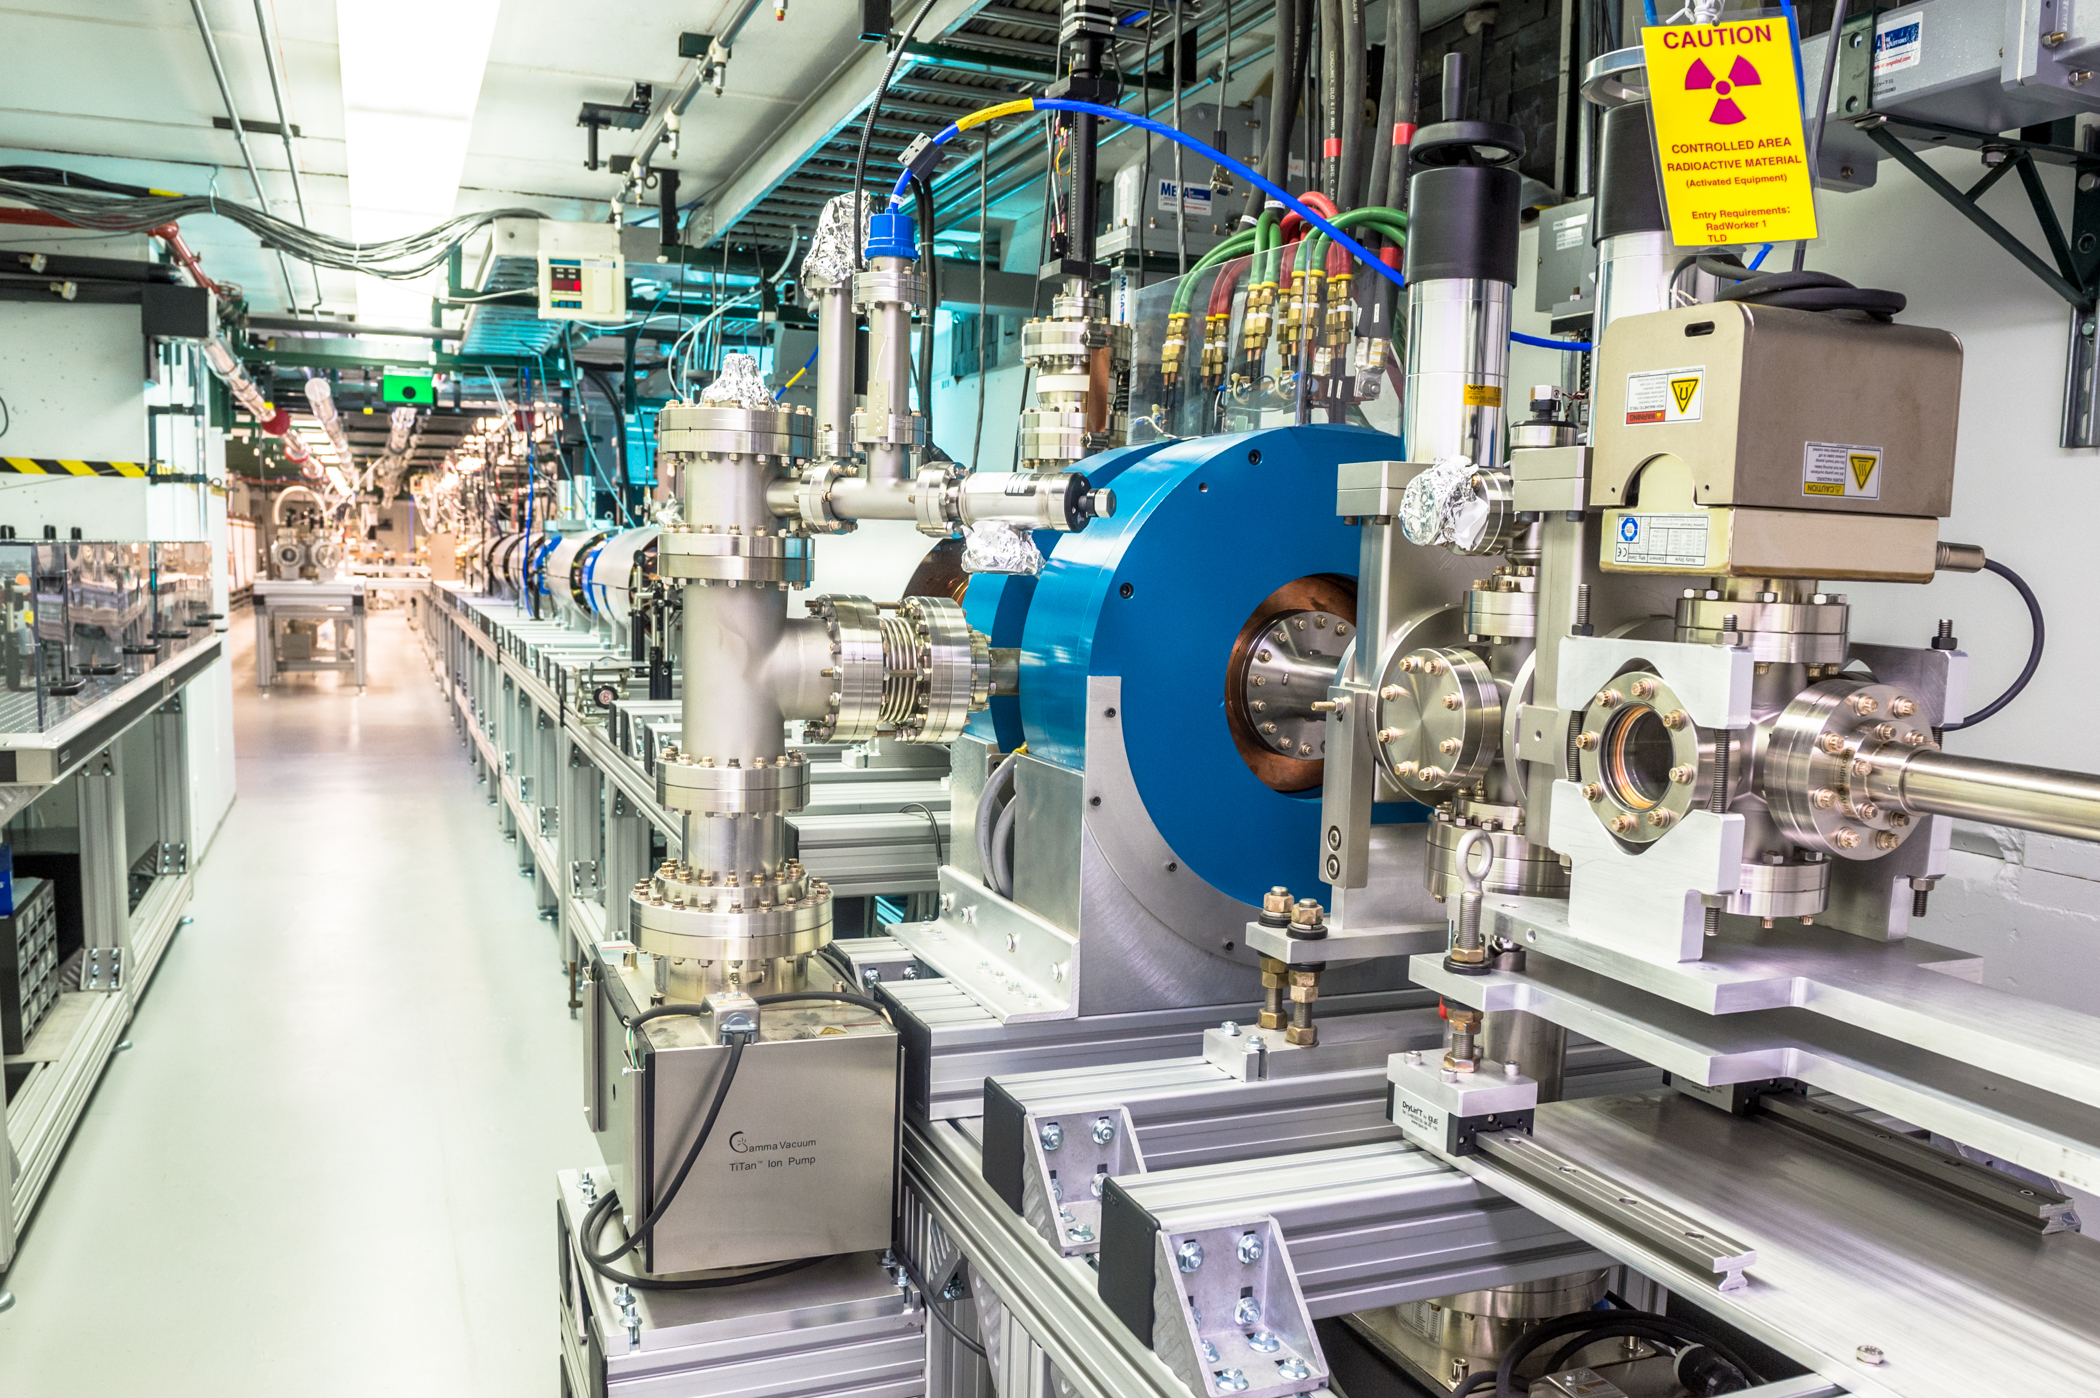
\includegraphics[width=1.0\linewidth, right]{../images/drive_gun}
	\end{column}%
\end{columns}
\end{frame}
%%%%%%%%%%%%%%%%%%%%%%%%%%%%%%%%%%%%%%%%%%%%%%%%%%%%%%%%%%%%%%%%%%%%%%%%%%%%%%%%
\subsection{Ongoing Experiments}
\begin{frame}
	\frametitle{AWA Facility}
	%\vspace{-1em}
	Current experiments include:
	\begin{itemize}
		\item{Emittance Exchange (EEX)}
		\item{Electron Radiography Imaging (ERI)}
		\item{Cathode Studies}
	\end{itemize}
	\vspace{0.3cm}
	\centering
	%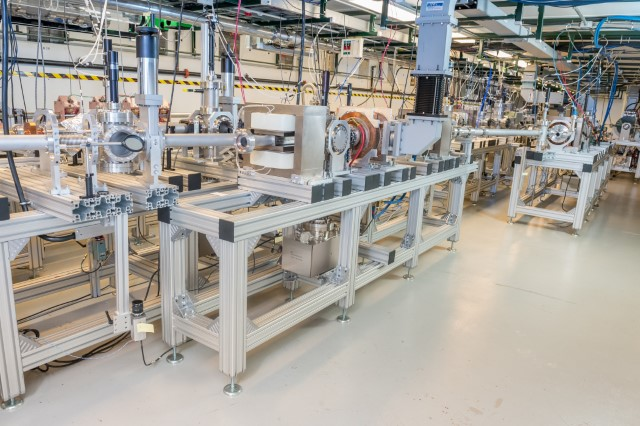
\includegraphics[width=0.5\linewidth]{../images/EEX}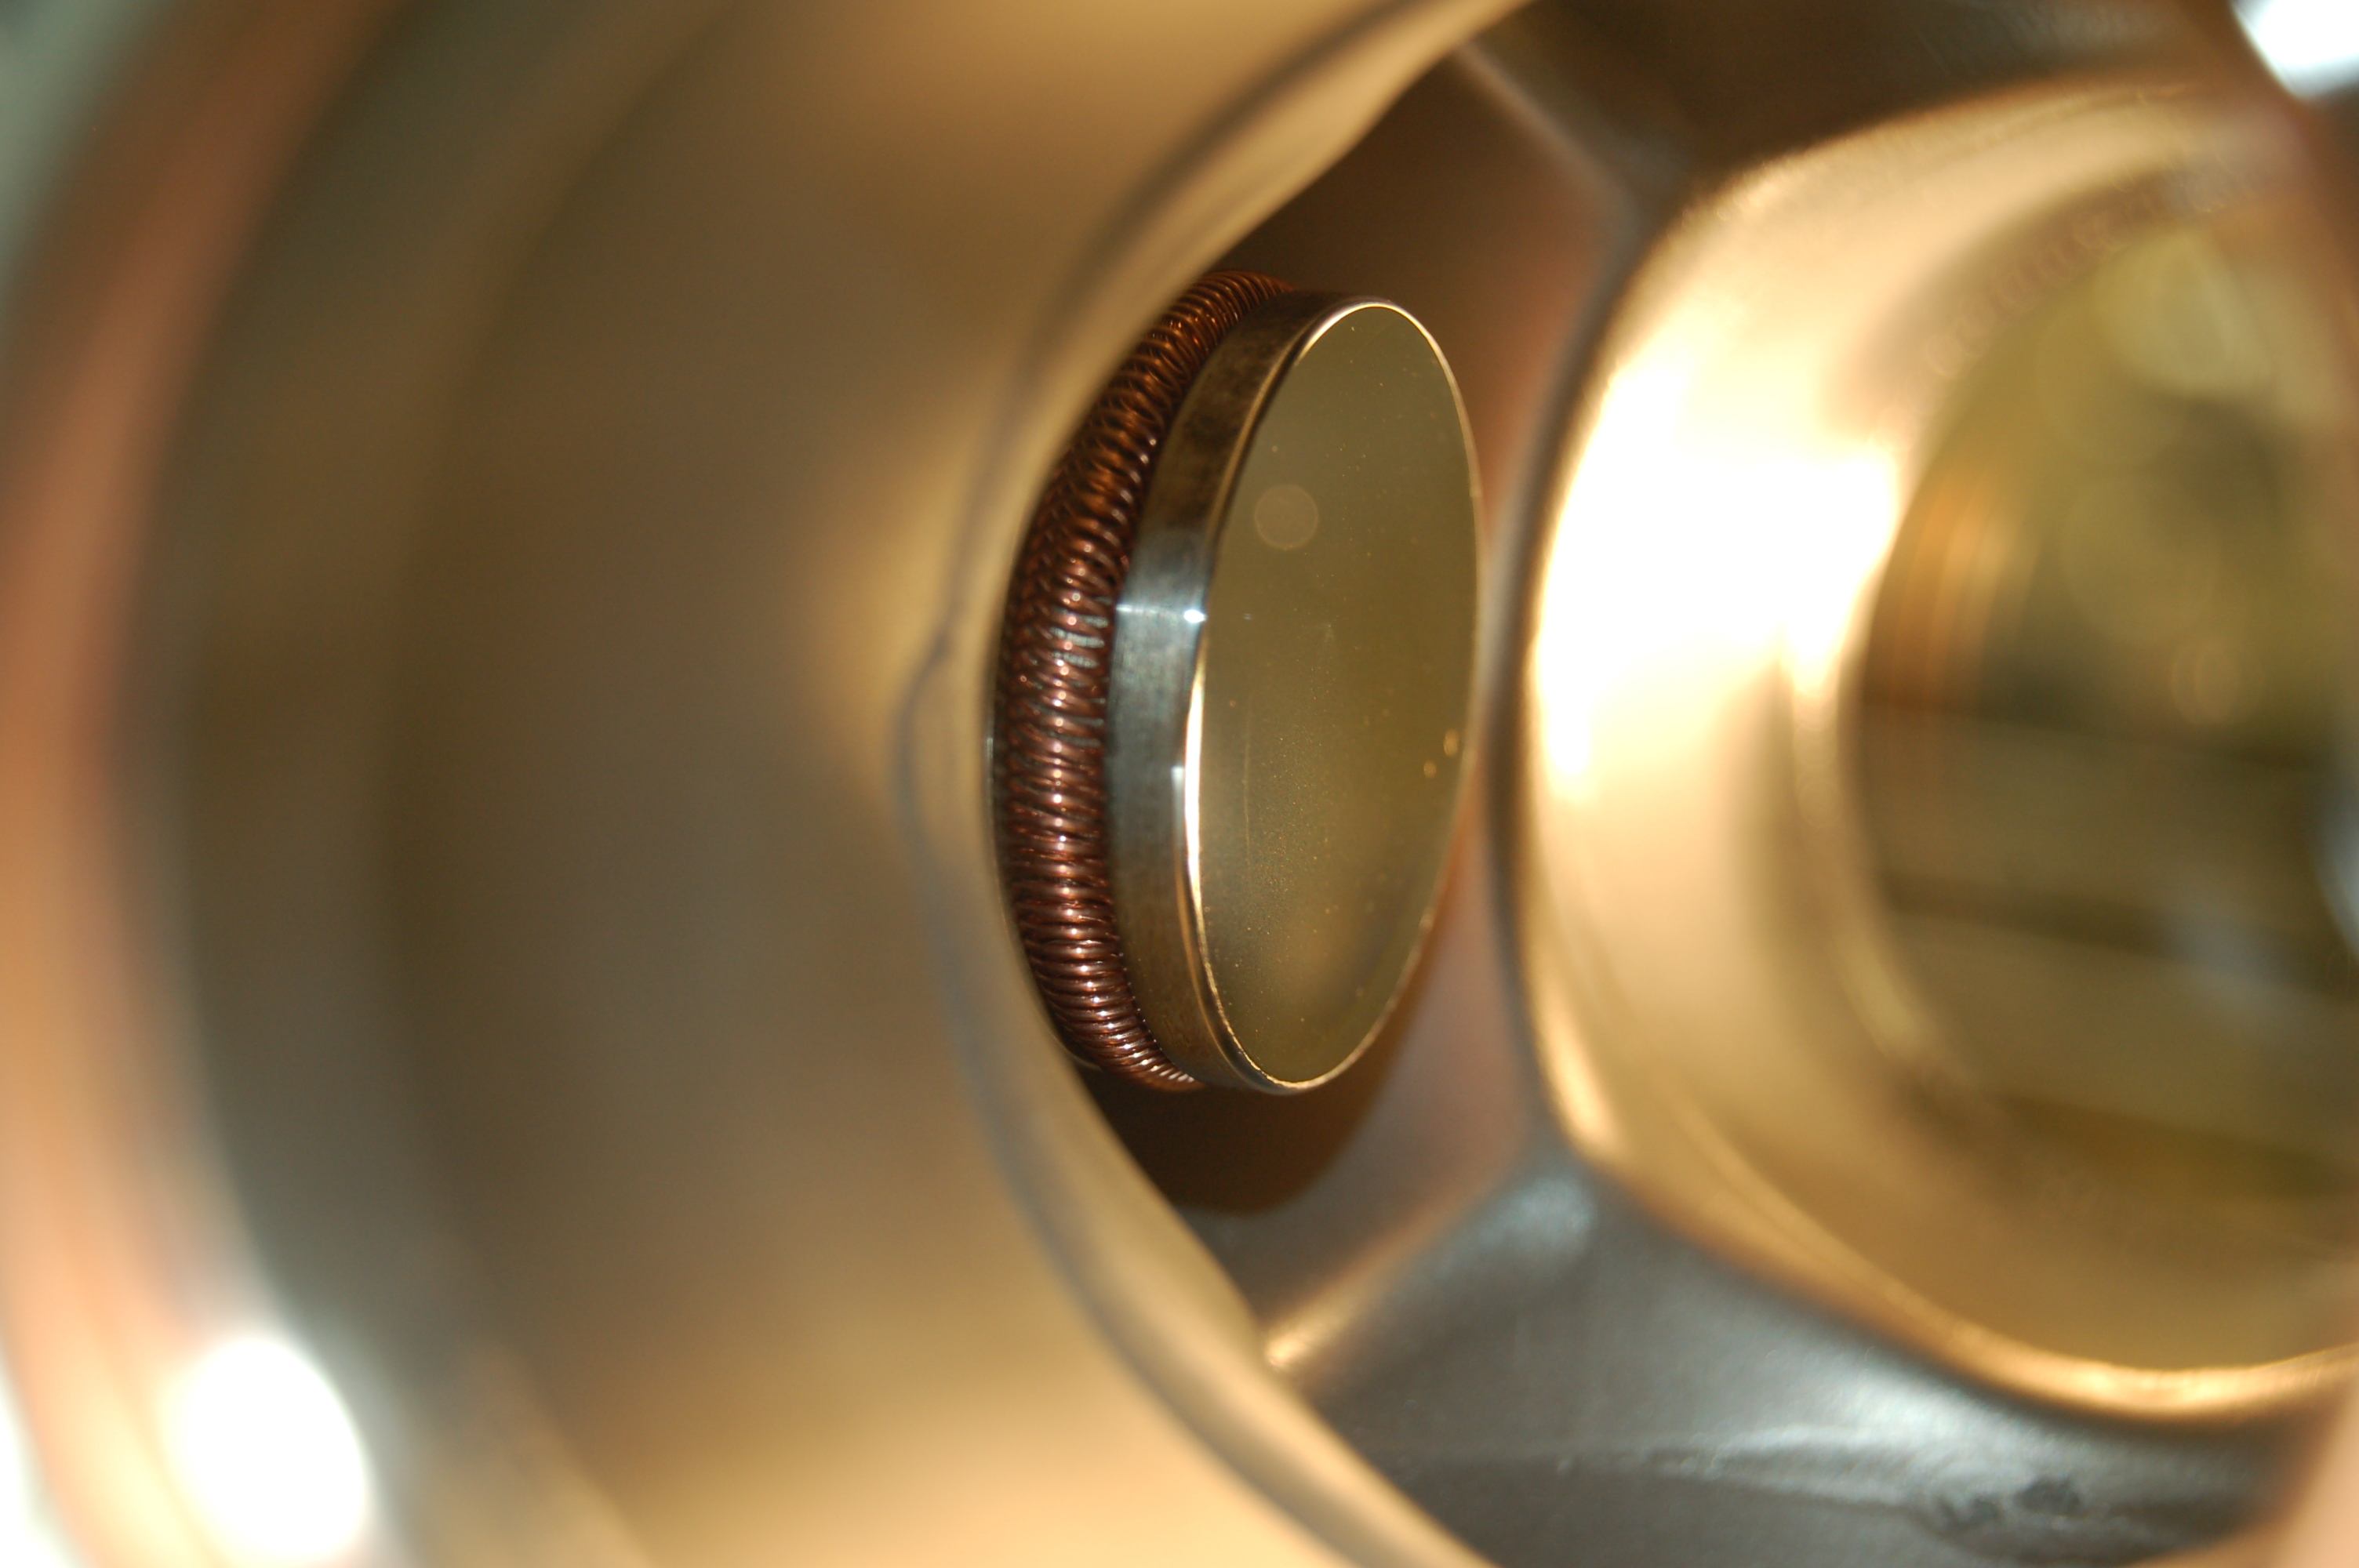
\includegraphics[width=0.5\linewidth]{../images/cathode1}
\end{frame}
%%%%%%%%%%%%%%%%%%%%%%%%%%%%%%%%%%%%%%%%%%%%%%%%%%%%%%%%%%%%%%%%%%%%%%%%%%%%%%%%
\begin{frame}[t]
	\frametitle{AWA Facility}
	%\vspace{-1em}
	Current experiments include:
	\begin{itemize}
		\item{Two Beam Acceleration (TBA)}
		\item{Beam line design for TBA = my thesis}
		\item{Dielectric accelerating and decelerating structure tests}	
	\end{itemize}
    \vspace{1em}
    % for trim = left, lower, right, upper
	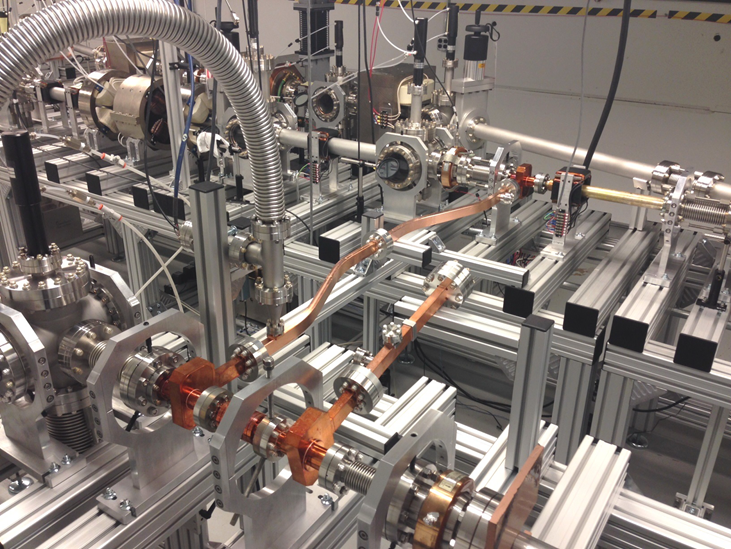
\includegraphics[width=0.5\linewidth, trim={0 0 0 1.65cm},clip]{../images/stage}\hfill%
	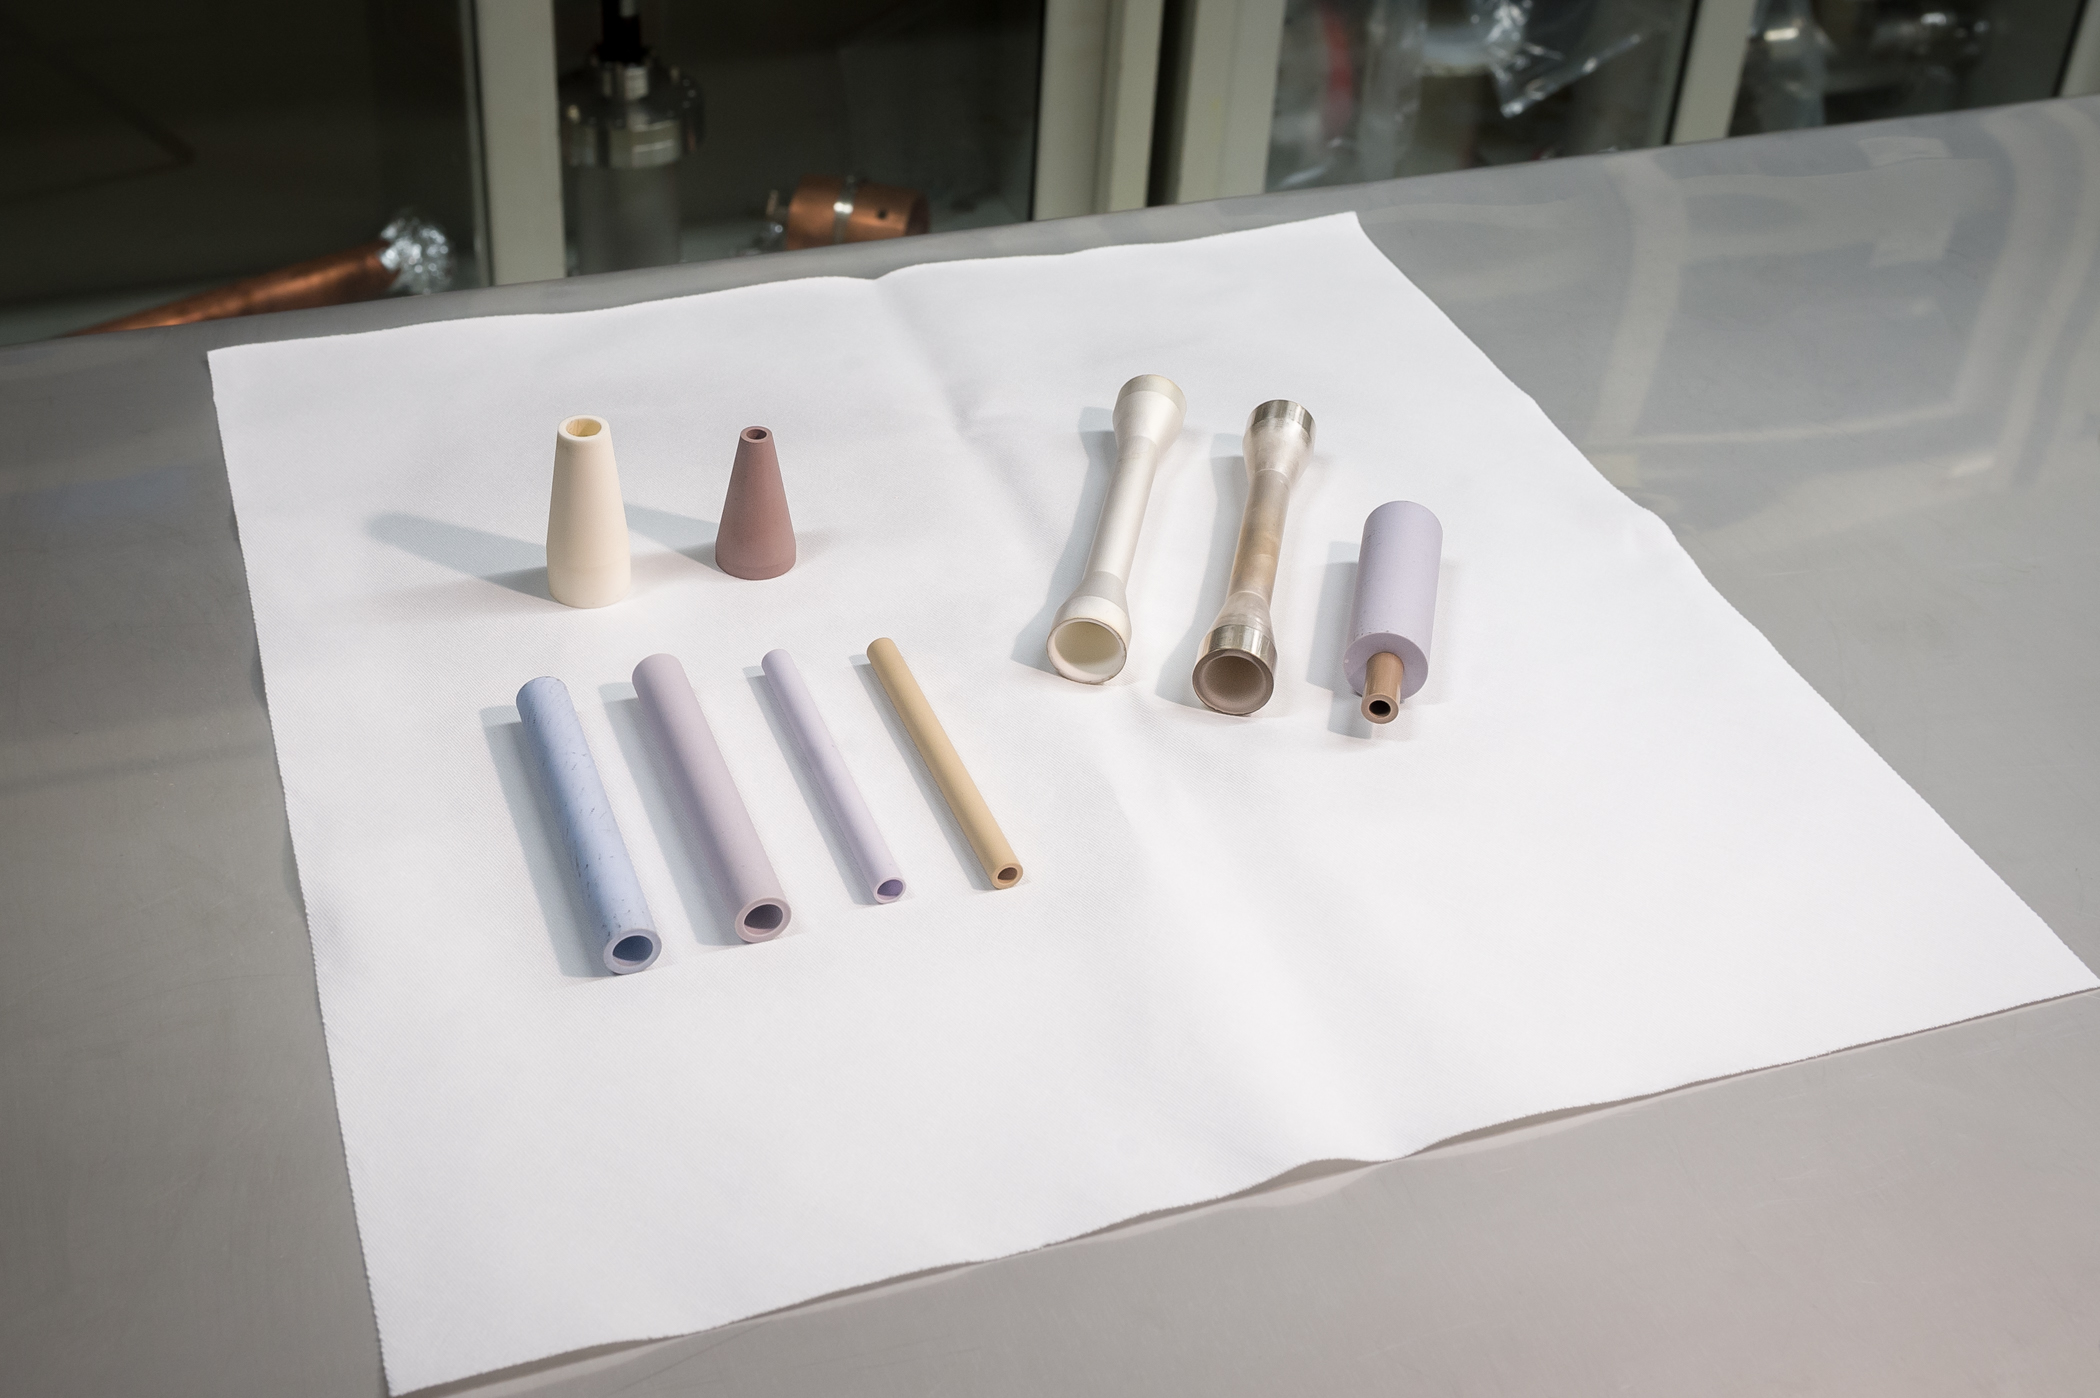
\includegraphics[width=0.5\linewidth]{../images/dielectrics}	
\end{frame}
%%%%%%%%%%%%%%%%%%%%%%%%%%%%%%%%%%%%%%%%%%%%%%%%%%%%%%%%%%%%%%%%%%%%%%%%%%%%%%%%
\section{Simulations}
\subsection{Code}
\begin{frame}[containsverbatim]
\frametitle{Code}
OPAL-T: \begin{verbatim}
	https://gitlab.psi.ch/OPAL/src/wikis/home
\end{verbatim}
\begin{itemize}
\item Developed at PSI
\item Free, open source 
\item Easy to work with developers
\item Parallel (scales....)
\item Features include 3D space charge and wakefields
\item RF photoinjector benchmark:
\end{itemize}
\begin{verbatim}
https://gitlab.psi.ch/OPAL/src/wikis/RFPhotoInjector
\end{verbatim}
\end{frame}
%%%%%%%%%%%%%%%%%%%%%%%%%%%%%%%%%%%%%%%%%%%%%%%%%%%%%%%%%%%%%%%%%%%%%%%%%%%%%%%%
\subsection{Optimization}
\begin{frame}
	\frametitle{Optimization (Linac only)}
	\Wider[4em]{
		\begin{minipage}{0.6\textwidth}
			Goals:
			\begin{itemize}

				\item{Determine what emittance and bunch length we can expect from the linac}
				\item{Determine optimum settings for TBA experiments}
				\item{Varied 10 parameters:}
			\end{itemize}
		\end{minipage}%
		\begin{minipage}{0.4\textwidth}
			\def \gunleft {-1.0}
			\def \gunright {0.3}
			\def \loneright {1.0}
			\def \ltworight {2.0}
			\def \lthreeright {3.0}
			\def \lfourright {4.0}
			\def \lfiveright {5.0}
			\def \lsixright {6.0}
			\centering
			\begin{center}
				\begin{tikzpicture}[scale=0.55]%,use optics
				%Gun drawings
				\draw[fill=orange, very thick, rounded corners =0.1cm] (\gunleft-0.2,0.5)rectangle (\gunright,1.5) node[pos=.5, white] {\textbf{Gun}} ;
				
				%S1
				\node[] at (-1.5,2.9) {$S_1$};
				\draw[ultra thick, fill=black!60!green] (-1.4,-0.5)rectangle  (-1.0,0.5) node[pos=.5, white] {} ;
				\draw[black, ultra thick] (-1.4,-0.5) -- (-1.0,0.5);
				\draw[black, ultra thick] (-1.4,0.5) -- (-1.0,-0.5);
				\draw[ultra thick, fill=black!60!green] (-1.4,1.5)rectangle  (-1.0,2.5) node[pos=.5, white] {} ;
				\draw[black, ultra thick] (-1.4,1.5) -- (-1.0,2.5);
				\draw[black, ultra thick] (-1.4,2.5) -- (-1.0,1.5);
				%S2
				\node[] at (-0.8,2.9) {$S_2$};
				\draw[ultra thick, fill=black!60!green] (-1.0,-0.5)rectangle  (-0.6,0.5) node[pos=.5, white] {} ;
				\draw[black, ultra thick] (-1.0,-0.5) -- (-0.6,0.5);
				\draw[black, ultra thick] (-1.0,0.5) -- (-0.6,-0.5);
				\draw[ultra thick, fill=black!60!green] (-1.0,1.5)rectangle  (-0.6,2.5) node[pos=.5, white] {} ;
				\draw[black, ultra thick] (-1.0,1.5) -- (-0.6,2.5);
				\draw[black, ultra thick] (-1.0,2.5) -- (-0.6,1.5);
				
				%S3
				\node[] at (0.2,2.9) {$S_3$};
				\draw[ultra thick, fill=black!60!green] (-0.1,-0.5) rectangle  (0.3,0.5) node[pos=.5, white] {};
				\draw[black, ultra thick] (-0.1,-0.5) -- (0.3,0.5);
				\draw[black, ultra thick] (-0.1,0.5) -- (0.3,-0.5);
				\draw[ultra thick, fill=black!60!green] (-0.1,1.5) rectangle  (0.3,2.5) node[pos=.5, white] {};
				\draw[black, ultra thick] (-0.1,1.5) -- (0.3,2.5);
				\draw[black, ultra thick] (-0.1,2.5) -- (0.3,1.5);
				%Linac drawings 
				\draw[fill=blue, ultra thick, rounded corners =0.1cm] (\loneright,0)rectangle  ({\loneright+0.84},2) node[pos=.5, white] {$L_1$} ;
				\draw[fill=blue, ultra thick, rounded corners =0.1cm] (\ltworight,0)rectangle  ({\ltworight+0.84},2) node[pos=.5, white] {$L_2$};
				\draw[fill=blue, ultra thick, rounded corners =0.1cm] (\lthreeright,0)rectangle ({\lthreeright+0.84},2) node[pos=.5, white] {$L_3$};
				\draw[fill=blue, ultra thick, rounded corners =0.1cm] (\lfourright,0)rectangle ({\lfourright+0.84},2) node[pos=.5, white] {$L_4$};
				\draw[fill=blue, ultra thick, rounded corners =0.1cm] (\lfiveright,0)rectangle ({\lfiveright+0.84},2) node[pos=.5, white] {$L_5$};
				\draw[fill=blue, ultra thick, rounded corners =0.1cm] (\lsixright,0)rectangle ({\lsixright+0.84},2) node[pos=.5, white] {$L_6$};
				\end{tikzpicture}
			\end{center}
		\end{minipage}%
		\begin{center}
			\setcounter{mpfootnote}{\value{footnote}}%
			\renewcommand{\thempfootnote}{\arabic{mpfootnote}}%	
			\begin{tabular}{ l *{3}{c}}
				%\toprule
				\textbf{Variable} & \textbf{Range} & \textbf{Unit} \\
				\midrule
				Solenoid Strength & $ 0 \le S_3 \le 440$  & amps \\
				Phase of Gun & $-60 \le \phi_g \le 60$  & degrees \\
				Laser Radius  & $0.1 \le R \le 30$  & mm \\
				Laser FWHM  & $2 \le T \le $10  & ps \\
				Cavity Phase & $-20 \le \phi_L \le 20$\footnote[1]{$\phi_L=[\phi_{L_1},\ldots,\phi_{L_6}]$} & degrees
				%\bottomrule    
			\end{tabular}
		\end{center}
	}
\end{frame}
\begin{frame}
	\frametitle{Ongoing Optimization Efforts}
\begin{columns}[T] % align columns
	\begin{column}{.56\textwidth}
		\vspace{1em}
		%\color{red}\rule{\linewidth}{4pt}		
		%\color{blue}\rule{\linewidth}{4pt}
		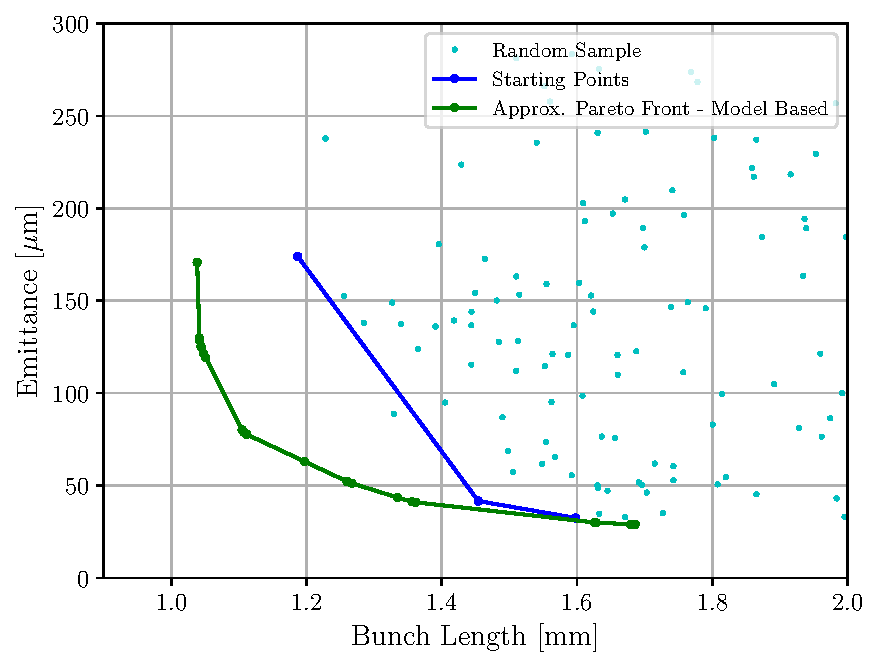
\includegraphics[width=1.0\linewidth, right]{../images/pareto_emittance_vs_zrms}
	\end{column}%
	\hfill%
	\begin{column}{.44\textwidth}
		\vspace{1em}
		Code verifies:
		\begin{itemize}
		\item Larger laser radius is always better
		\item Shorter laser pulse length $\rightarrow$ shorter $\sigma_z$
		\item Longer laser pulse $\rightarrow$ lower $\epsilon_{x,y}$
	    \end{itemize}	
	\end{column}%
\end{columns}
\end{frame}
%%%%%%%%%%%%%%%%%%%%%%%%%%%%%%%%%%%%%%%%%%%%%%%%%%%%%%%%%%%%%%%%%%%%%%%%%%%%%%%%
\section{Experimental Measurements}
\subsection{Overview}
\begin{frame}
Took data 1.5 weeks ago!

Tried to dial in machine settings based on simulations:
\begin{itemize}
	\item Initial results did not match simulations - not a surprise
	\item Identified problems with machine parameters:
	\begin{itemize}
		\item Solenoid strength
		\item Energy 
	\end{itemize}
	
	
	\item Adjusted settings to approach simulation values
	\item Took three types of data:
	\begin{itemize}
		\item Beam size data - YAG screens
		\item Emittance - scanning slit
		\item Bunch length - CTR, interferometer, and, bolometer 
	\end{itemize}
\end{itemize}
%\includegraphics[width=0.25\linewidth]{YAG1}\includegraphics[width=0.25\linewidth]{YAG2}%
%\includegraphics[width=0.25\linewidth]{YAG3}\includegraphics[width=0.25\linewidth]{YAG3}

\end{frame}
%%%%%%%%%%%%%%%%%%%%%%%%%%%%%%%%%%%%%%%%%%%%%%%%%%%%%%%%%%%%%%%%%%%%%%%%%%%%%%%%
\subsection{Measurements}
\begin{frame}
	\frametitle{Beam Size Measurements}
	\vspace{-1em}
\begin{columns}[T] % align columns
	\begin{column}{.5\textwidth}
		%\color{red}\rule{\linewidth}{4pt}		
		2D Results:
    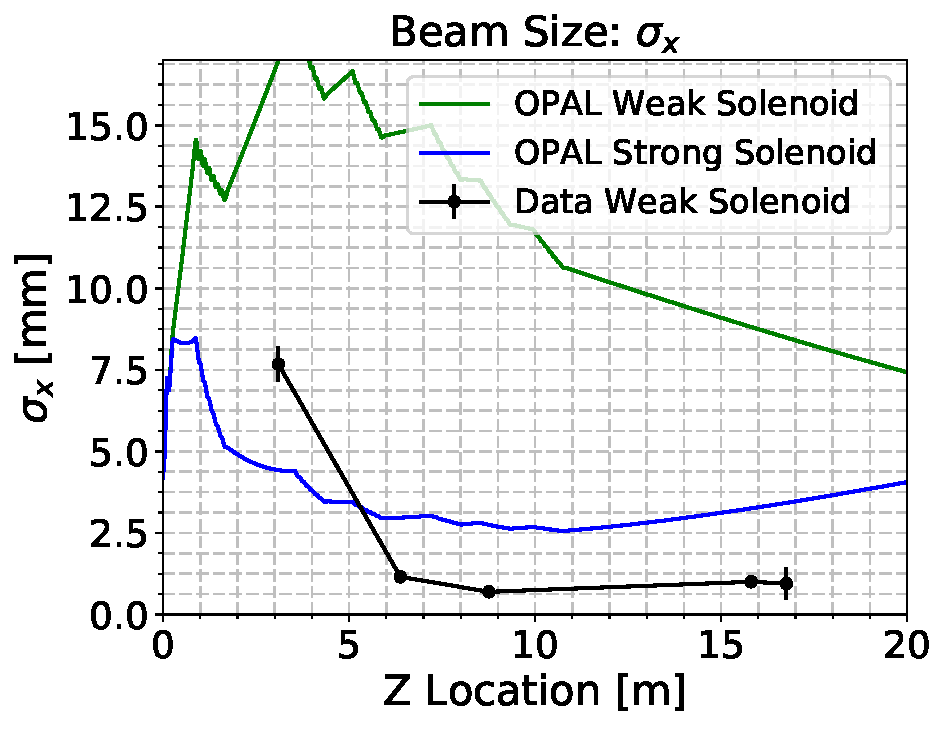
\includegraphics[width=0.75\linewidth]{../images/beamsizes_2Dx} \\ \vspace{0.25em}
    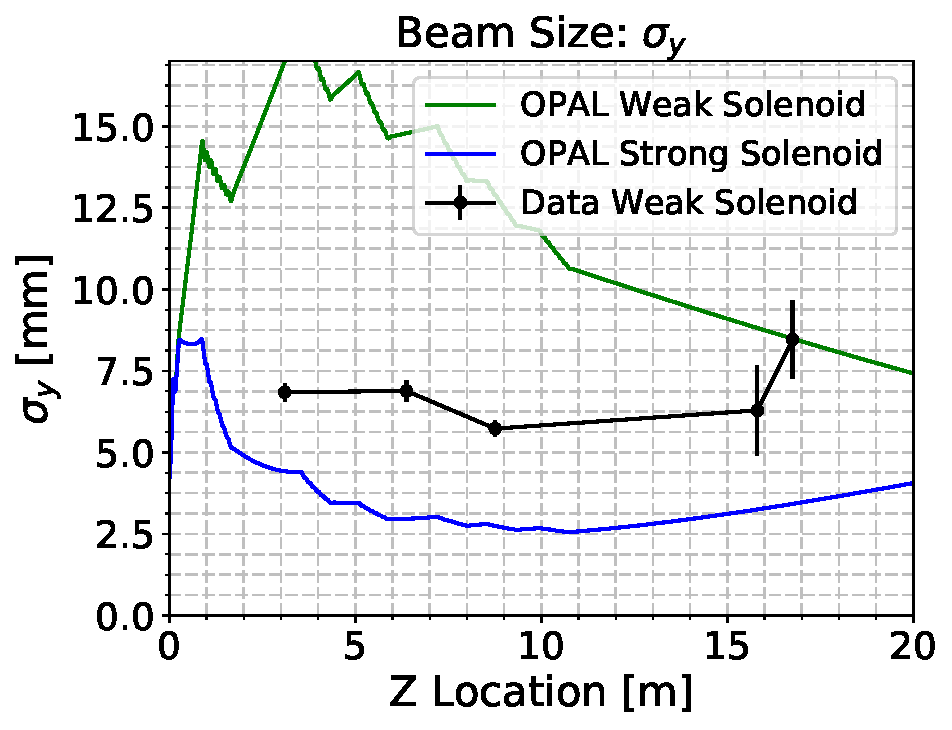
\includegraphics[width=0.75\linewidth]{../images/beamsizes_2Dy}
	\end{column}%
	\hfill%
	\begin{column}{.5\textwidth}
		%\vspace{1em}
		%\color{blue}\rule{\linewidth}{4pt}
		3D Results:
		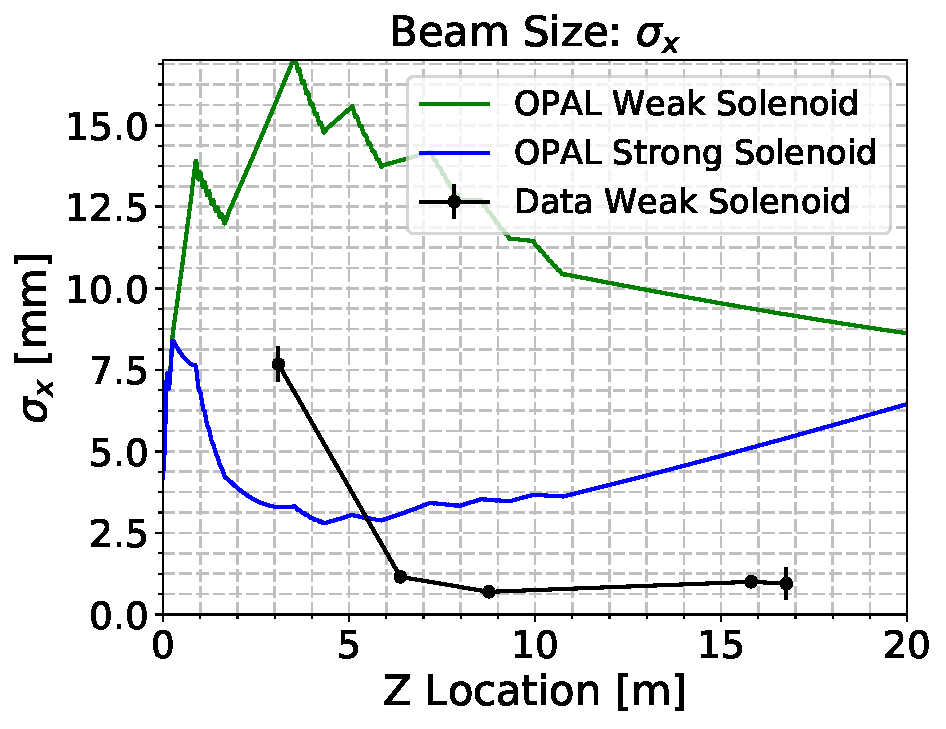
\includegraphics[width=0.75\linewidth]{../images/beamsizes_3Dx} \\ \vspace{0.25em}
		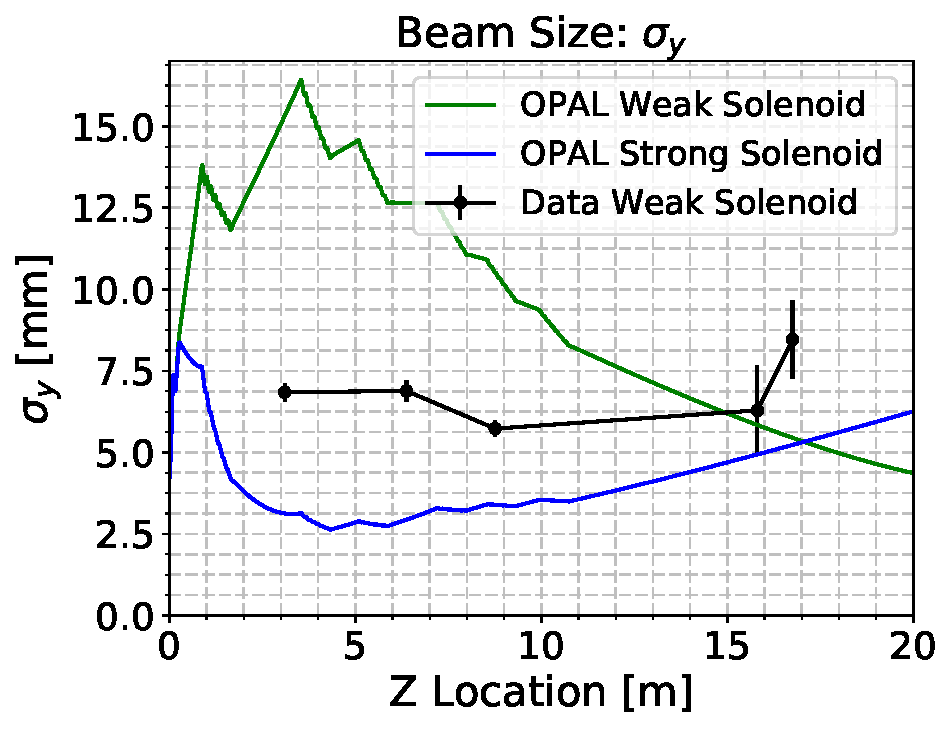
\includegraphics[width=0.75\linewidth]{../images/beamsizes_3Dy}
	\end{column}%
\end{columns}
\end{frame}
%%%%%%%%%%%%%%%%%%%%%%%%%%%%%%%%%%%%%%%%%%%%%%%%%%%%%%%%%%%%%%%%%%%%%%%%%%%%%%%%
\begin{frame}
	\frametitle{Summary}
	Goal: Use simulations to optimize beam parameters. 
	\begin{itemize}
		
		\item AWA configuration is constantly changing
		\item Build a set of tools to quickly optimize between beam setting
		\item Use agreement between simulations and measurements to guide experiments
	
	\end{itemize}
\end{frame}
%%%%%%%%%%%%%%%%%%%%%%%%%%%%%%%%%%%%%%%%%%%%%%%%%%%%%%%%%%%%%%%%%%%%%%%%%%%%%%%%
\begin{frame}
\vspace{5em}
\Huge {Thanks for your time!} \\ 
%\normalfont{And thanks to my funding sources:}
\includegraphics[width=0.5\linewidth]{../images/IIT_Logo_blk-eps-converted-to} %\\%

\includegraphics[width=0.5\linewidth]{../images/Argonne_cmyk_black}%
%
\includegraphics[width=0.5\linewidth]{../images/DOE_logo_color_cmyk}
\\
\end{frame}


\end{document}
















